\documentclass[14pt, a4paper]{book}
\begin{document}\label{chap:Method_ML}
We have now presented the dataset and theory behind everything, and are thus ready to start making our ML algorithms. The first part of this chapter will be a presentation of the dataset in more details, included all the events and the difficult variable called the \textit{weights}.
We will also explore how we divide our dataset into a training and testing set. Afterwards we will discuss the crucial task of optimizing the architecture and hyperparameters of the ML models for obtaining high-performance classifiers. In this field, the challenge is often to 
distinguish between signal events from rare physics phenomena, such as our DM interactions, and the much more common SM background events. Since these signals events are extremely rare, the classifiers need to be highly optimized in order to effectively separate them from 
the background. In addition, the datasets have a large number of features, which can lead to overfitting or poor generalization if not properly optimized. Another hardship is how to mitigate the phenomena of jagged arrays and missing variables described in the previous chapter.\\
\\It is therefore essential to carefully choose the model architecture and hyperparameters, as well as the dataset pre-processing techniques, in order to achieve the best possible performance in the search for the rare DM physics phenomena. This can involve optimizing 
parameters such as the learning rate, the regularization strength, (exclusively for the NNs) the number of layers, the number of neurons per layer, (exclusively for the BDTs) the number of trees, and the tree depth. The second and third part of this chapter will be just about optimization for the NNs and BDTs respectively.

\clearpage
\section{The datasets}
The way we are making datasets in this project, to keep it as close to model independent as possible, will be of the following format
\begin{itemize}
   \item Make a dataset with all of the SM backgrounds and one DM model.
   \item Make a dataset with all of the SM backgrounds and all of the DM models, divided into different signal regions.
\end{itemize}
The idea behind the first one is to start with a model dependent approach, where we train a ML algorithm to learn just one model at a time. The reason for taking this approach and not just having one dataset with all the models included, which would indeed make it 
a model independent approach, is because of the different phenomenology and experiemntal signatures of the models we are studying. \textbf{Question: Should I give concrete examples on how SUSY vs Z' differs, or is this sentence enough?} To achieve model indepence 
with this dataset, the plan is to combine the results of the different networks into one. \textbf{Question: Is it correct to say statisticslly combine the results? Or what exactly are we thinking of combining using this method?} \\
\\For the second one, even if we were to include models with different signatures it would work out in our favour. For example, if we created Signal Regions (SR) in different regions of the $m_{ll}$ phasespace, \textit{and} trained a ML network in each respective SR, 
then the network would learn the DM resonance appearing in each area, instead of learning the model resonance. Indeed, achieving model indepence. Furthermore, the plan is to combine the results of each respective region to get an overall view of all of Run II.\\
\\In this project we will look at real and simulated data from the ATLAS detector from all running periods of Run II. This is from period $a, d$ and $e$ each with an integrated luminosity of $36.4, 44.3$ and 58.5 $fb^{-1}$ respectively. 
In Table \ref{tab:dataset} we can see the overall number of MC samples and expected events for all background channels as well as DM models. In addition to using the features in Table \ref{tab:variables}, we will also include the EventID, dataset ID, period, 
dilepton final state, label telling us wether an event is signal or background and the \textit{weight} of each event.
\begin{table}[!h]
   \centering
    \caption[Dataset used for ML]{Table showcasing the number of MC samples and expected events for every background channel and DM model that will be used in this thesis.\\ * The expected number of events for any BSM model has prefixed assumptions about for example 
      cross section, decay width, etc. As we do not empirically know if any of these assumptions are correct, these are not set in stone.}
   \begin{tabular}{l|r|r}\midrule\midrule
      Channel                                                                         & MC samples            & Expected events  \\\midrule
      W                                                                               & 38,684                & 5,436.325        \\
      Drell Yan                                                                       & 47,201,697            & 2,198,257.648    \\
      TTbar                                                                           & 28,126,697            & 978,530.817      \\
      Single top                                                                      & 729,624               & 93,898.462       \\
      Diboson                                                                         & 10,983,689            & 116,653.466      \\\midrule
      Standard model total                                                            & 87,080,391            & 3,392,776.718    \\\midrule
      $Z'$ Dark Higgs Heavy Dark Sector                                               & 498,621               & *54.917         \\
      $Z'$ Dark Higgs Light Dark Sector                                               & 892,365               & *155.369         \\
      $Z'$ Light Vector Heavy Dark Sector                                             & 521,759               & *39.820         \\
      $Z'$ Light Vector Light Dark Sector                                             & 470,352               & *235.699         \\
      $Z'$ Effective Field Theory Heavy Dark Sector                                   & 715,409               & *0.0004           \\
      $Z'$ Effective Field Theory Light Dark Sector                                   & 640,963               & *0.0007          \\\midrule\midrule
   \end{tabular}
   \label{tab:dataset}
\end{table}

\subsection{Weights}\label{sec:wgts}
The weights are crucial for most of what is to come further on this thesis. The weights only apply to MC simulations and can be interpreted as corrections to simulate real data, which is why the MC samples and expected events on Table \ref{tab:dataset} differ, where the 
latter has applied weights. The weights on this project are defined as Eq. (\ref{eq:wgts}) and are in $fb^{-1}$ units.
\begin{equation}\label{eq:wgts}
   W = w_{mc}\times w_{pu}\times w_{xs}\times w_{lsf} \times w_{nlo,ew} \times w_{ttbar} \times w_{jet} \times w_{bjet} \times \frac{lumi_{period}}{\sum w_{mc, DSID}}
\end{equation}
This equation has a lot of information in it, so every part of this will be discussed. Starting from the raw MC weight, $w_{mc}$\\
The pile-up weight $w_{pu}$, takes into account detector featuers\\
The cross section weight $w_{xs}$, defined as $w_{xs} := xs \times w_{kf} \times g_{eff}$ where $xs$ is the cross section of the process, $w_{kf}$ is the $k-$factor which has higher order corrections, and $g_{eff}$ is the filter efficiency.\\
The Lepton and trigger Scale Factor (LSF), $w_{lsf}$, which...\\
The Next to Leading Order (NLO) electroweak correction $w_{nlo,ew}$, which ...\\
The $t\bar{t}$, jet and b-jet weights, $w_{ttbar}, w_{jet}$ and $w_{bjet}$, which ...\\
And lastly the luminosity of the period, meaning
$$
lumi_{period} = \begin{cases}
               36.4,& \text{for } period = a\\
               44.3,& \text{for } period = d\\
               58.5,& \text{for } period = e
               \end{cases}
$$
divided by the Sum Of Weights (SOW) \textbf{Question: Sum of every $w_{mc}$ of each event or sum of every $W$ pr event? } of every MC sample for each dataset ID (background process)

\subsection{Signal regions}
Will make three regions:\todo{Write in more details}
\begin{itemize}
   \item $m_{ll} >120$ GeV and $E_T^{miss} \in [50, 100]$ GeV
   \item $m_{ll} >120$ GeV and $E_T^{miss} \in [100, 150]$ GeV
   \item $m_{ll} >120$ GeV and $E_T^{miss} >150$ GeV
\end{itemize}



\subsection{Train and test split}\label{sec:train_test}
When training our networks we will use 80\% of the dataset, the remaining 20\% will be used to test whether the networks are learning any physical patterns or learning the dataset. When splitting the datasets however, we need to be absolutely certain that the distributions 
follow the same shape and have the same ratio of background channels as well as having good MC and data agreement. In this thesis we will utilize a function from \verb|scikit learn| \cite{scikit-learn} called \verb|train_test_split| which can easily split our dataset into 
a training and testing set of our size, while also sorting the label of the event. Another benefit of using this function is that is has included a random seed such that we can always split the datasets in the same shape.
\graphicspath{{../../../Plots/NeuralNetwork/FULL/}}
\begin{figure}[!ht]
	\centering
	\begin{subfigure}[b]{0.49\textwidth}
        \centering
        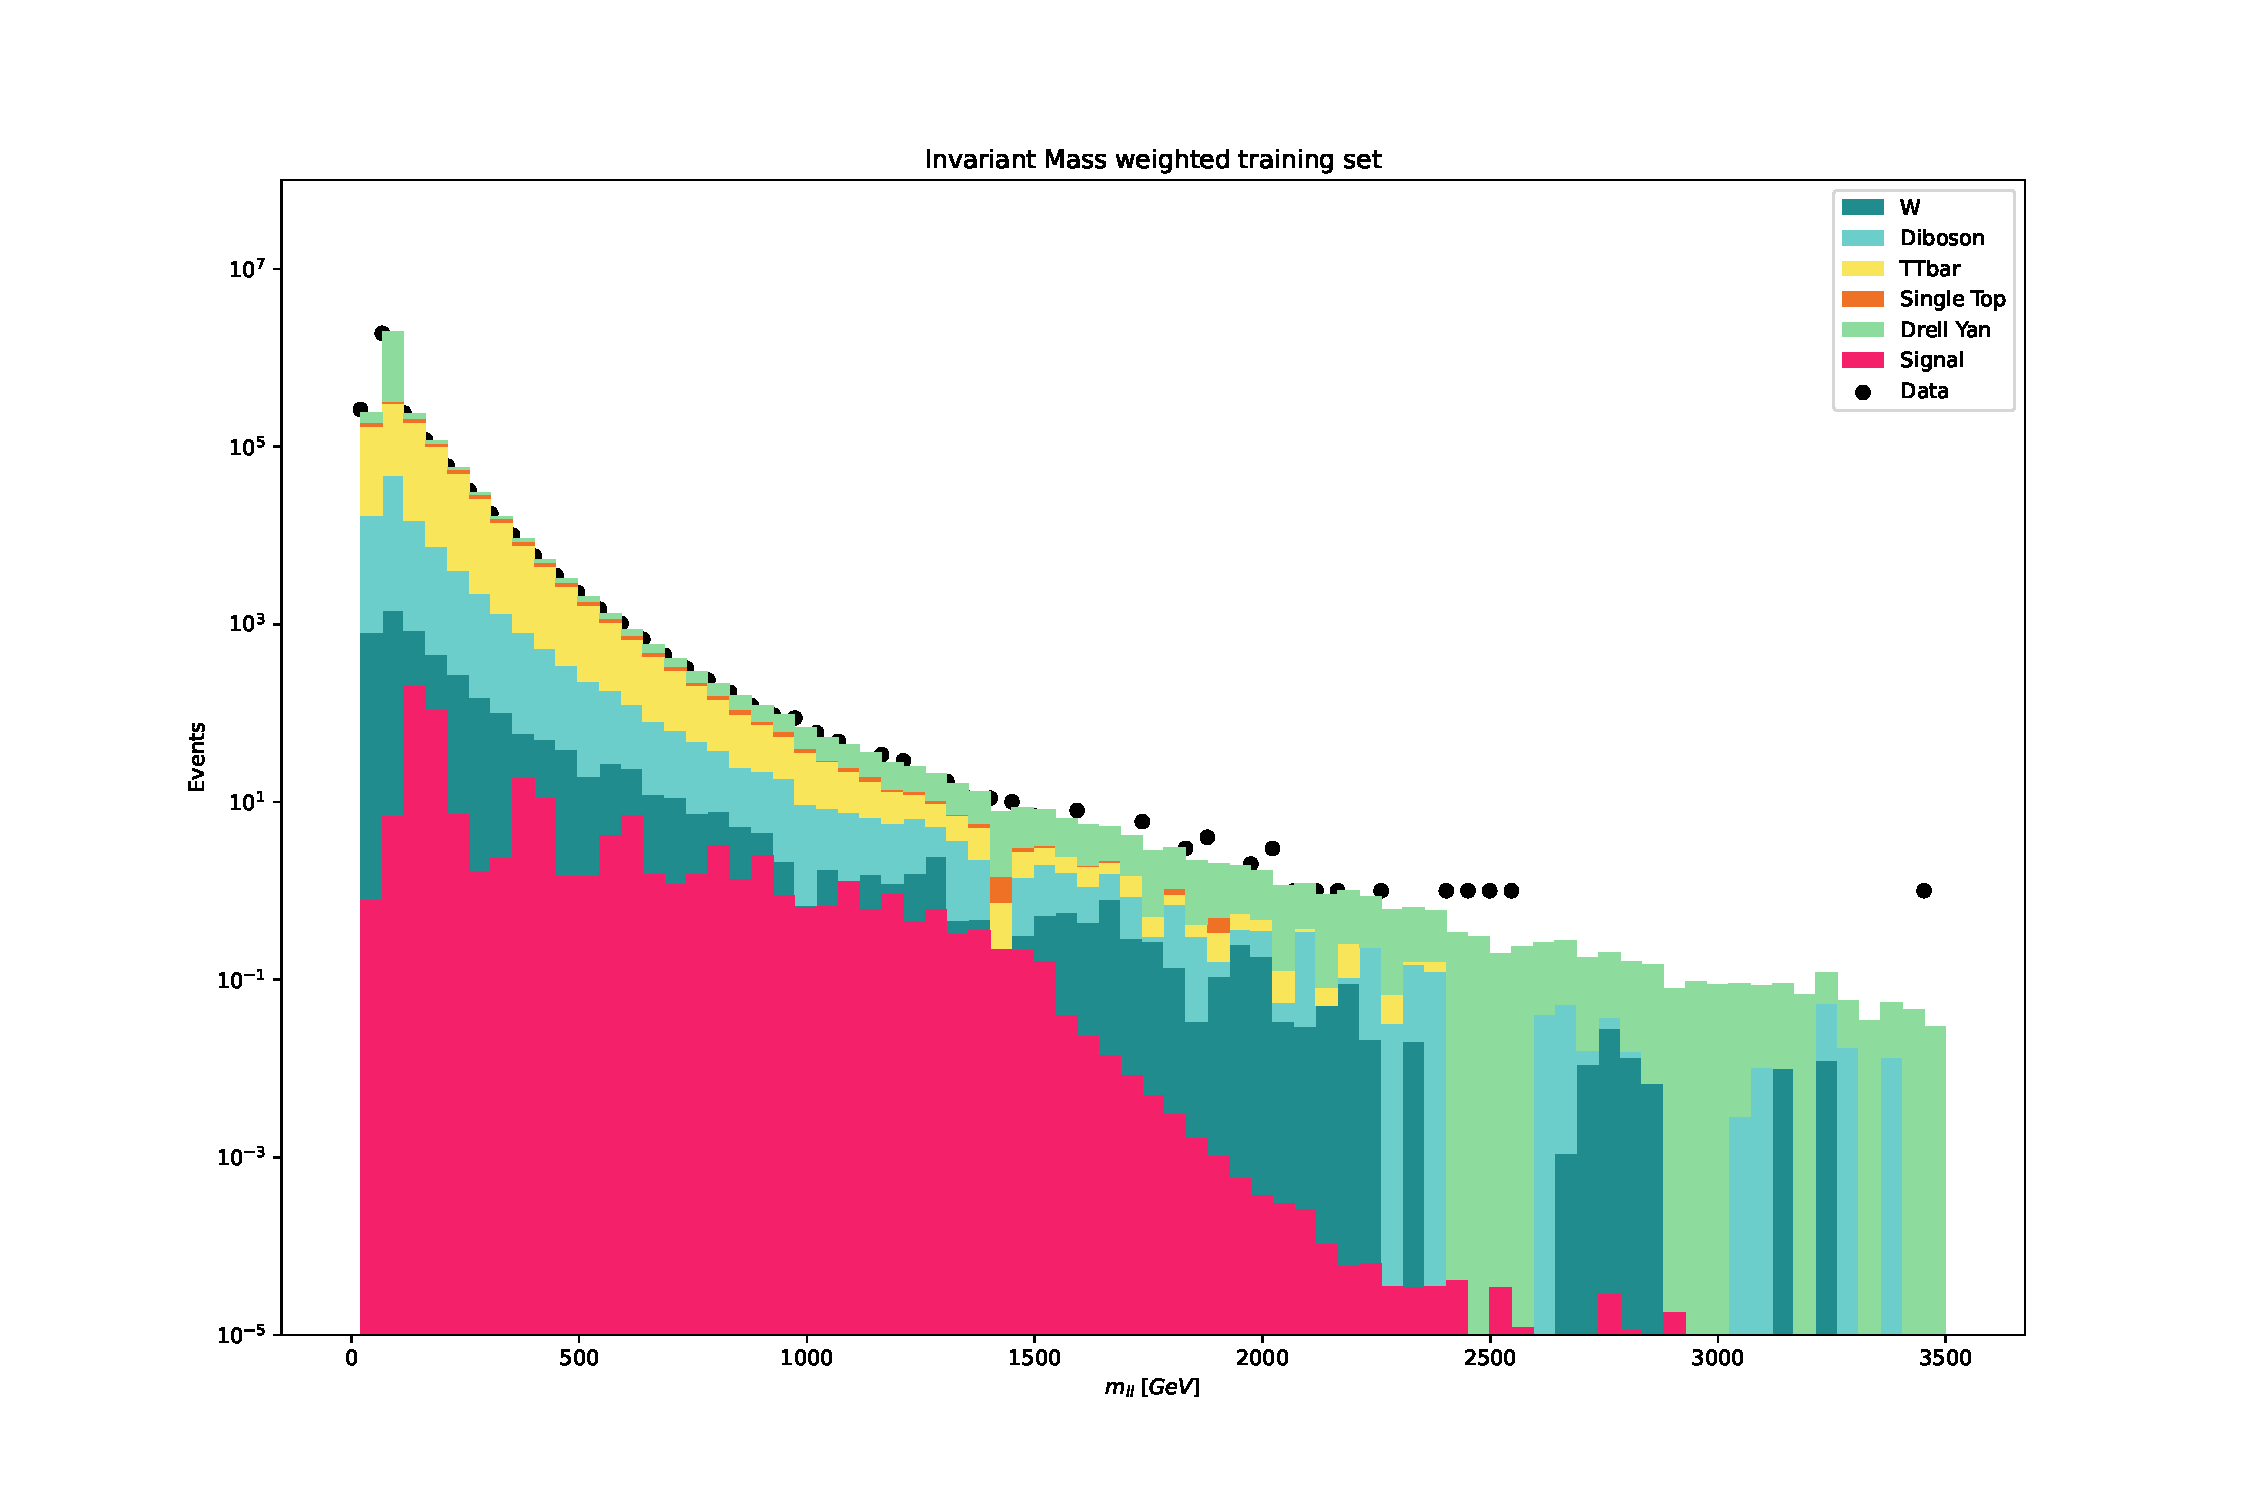
\includegraphics[width=1\textwidth]{mll_train.pdf}
        \caption{Training distribution}
     \end{subfigure}
     \hfill
     \begin{subfigure}[b]{0.49\textwidth}
        \centering
        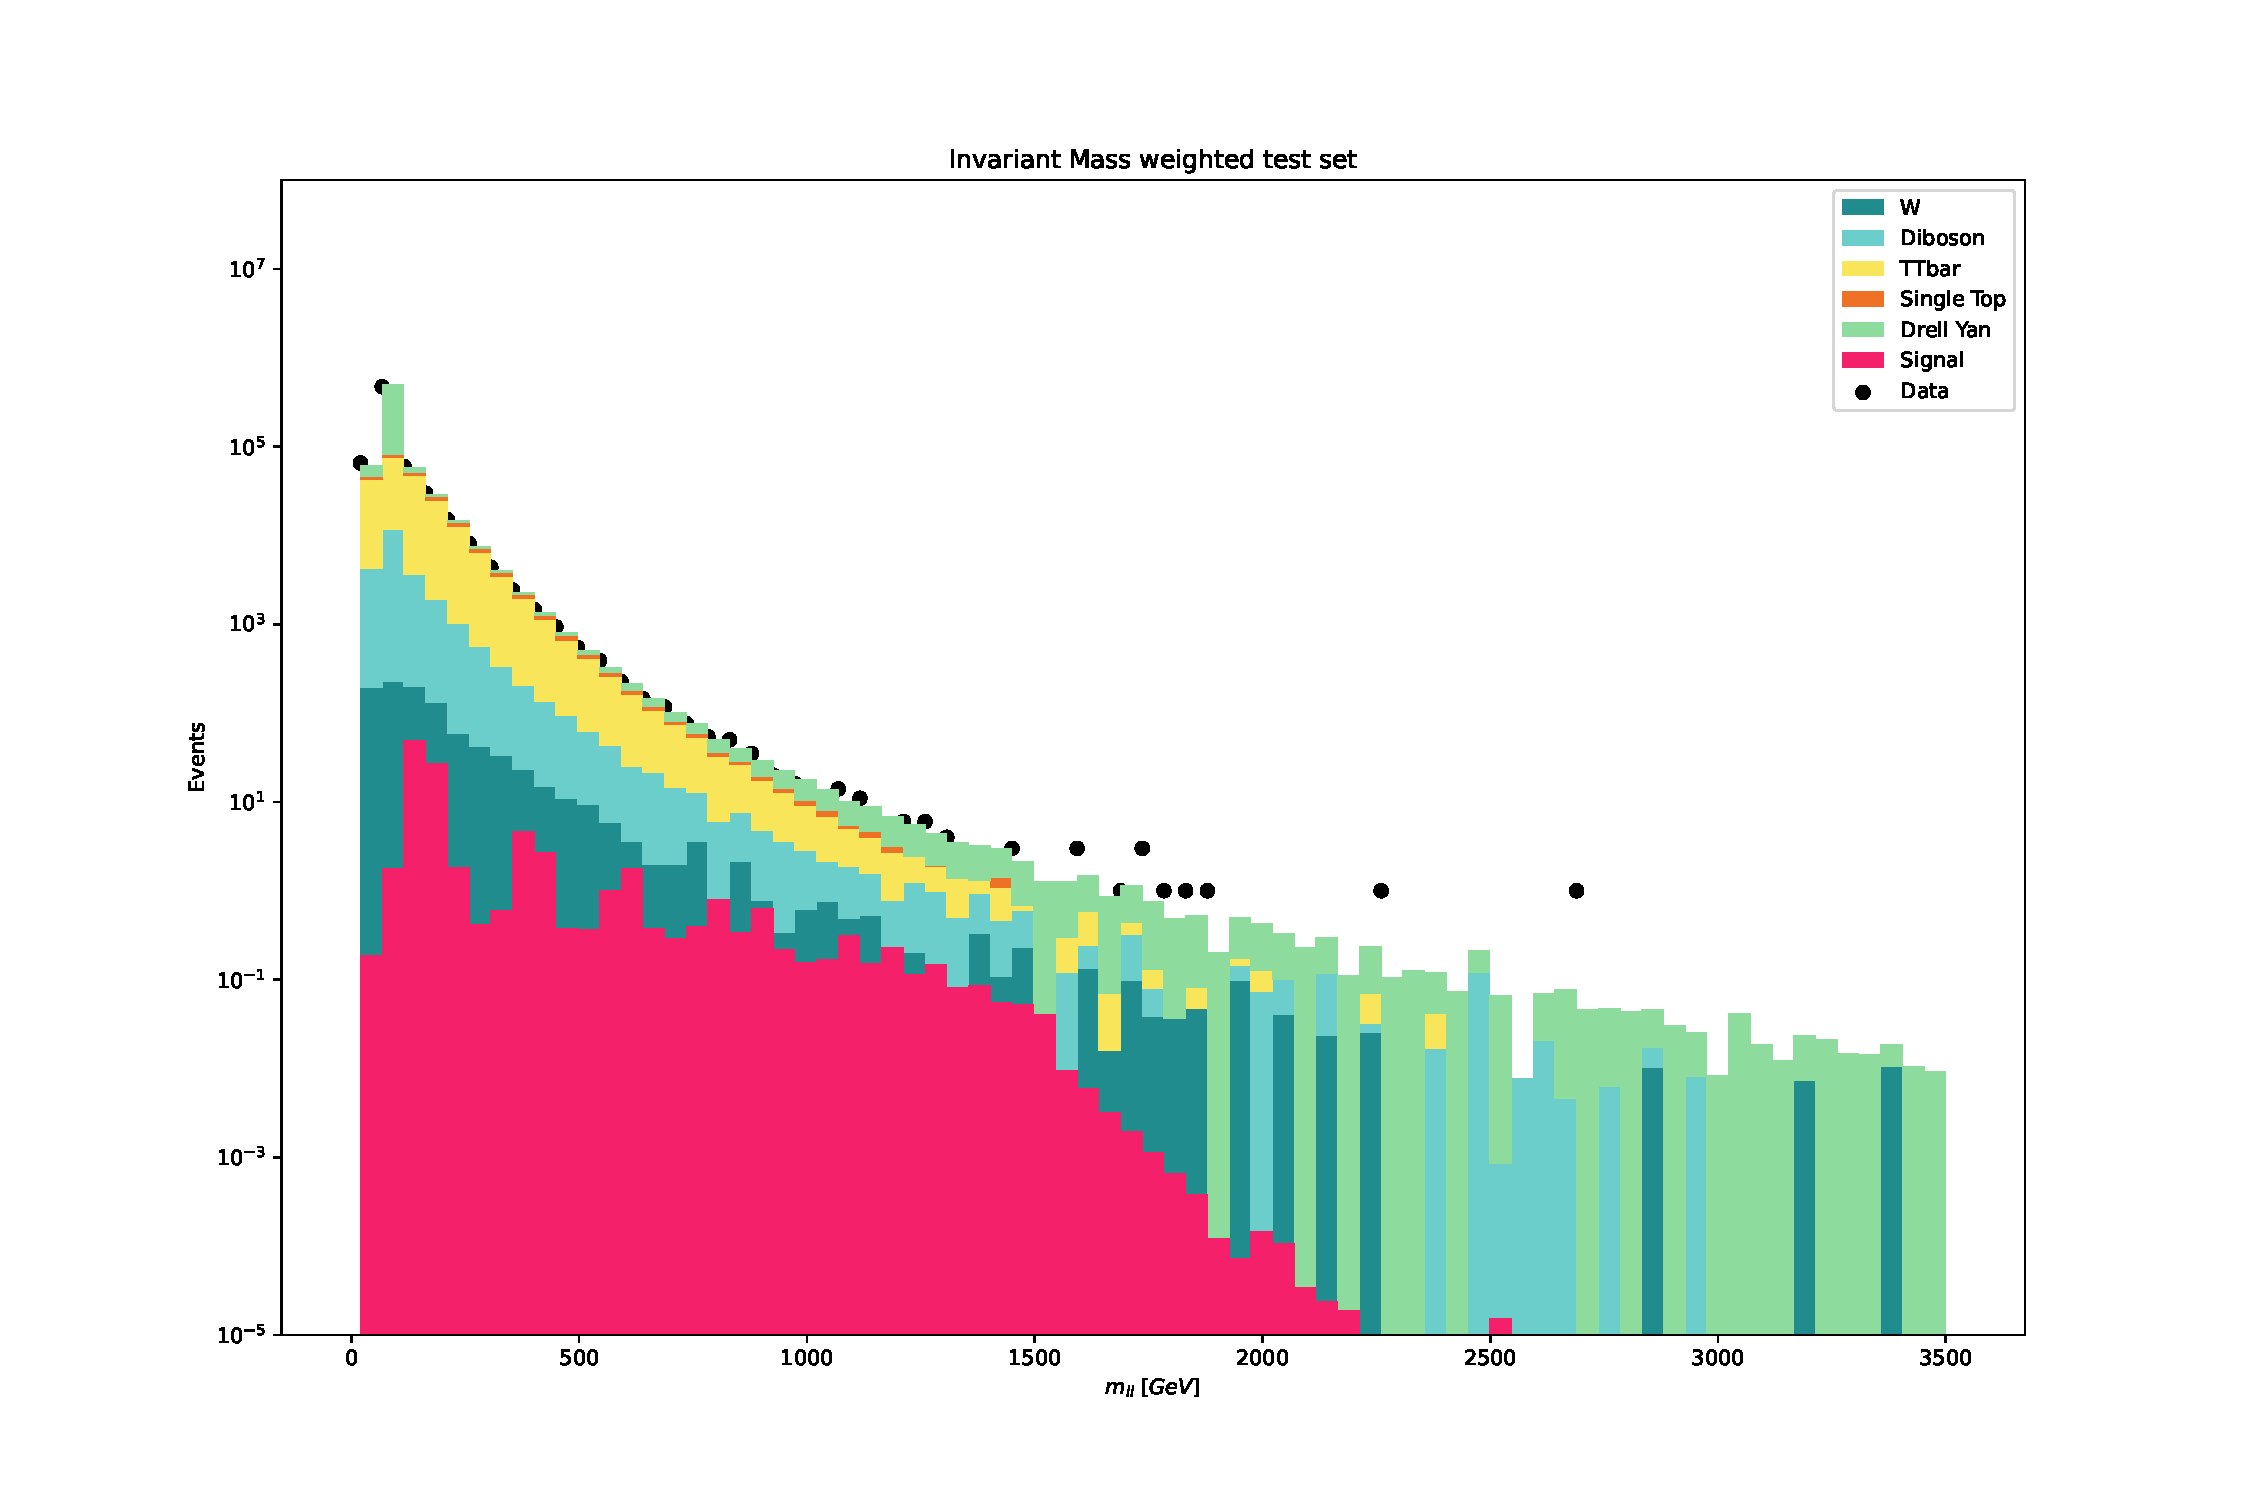
\includegraphics[width=1\textwidth]{mll_test.pdf}
        \caption{Testing distribution}
     \end{subfigure}
	\caption[Train-test split distribution]{Train and test distribution of the invariant mass when dividing SM background and DM samples}\label{fig:train-test}
\end{figure}
\\In Figure \ref{fig:train-test} \todo{add better figure} we can see that the distribution remains the same when we split the dataset into 80-20, where we also see the data and MC agree. To see the distribution of every other kinematical variable see \textbf{question: Appendix or github repo? The appendix is already very long!}
In addition to splitting the data, when making validation plots (See Chapter \ref{sec:validation}), when plotting MC simulations and real data, we nee to make sure that the luminosity of the plot is correct. That means that if we are plotting the network score in 
the test dataset, as this is 20\% of the whole dataset we need to scale everything with a factor of 5 so we get back to 100\% and the full luminosity of Run II.


\clearpage
\section{Neural Network Training}
For this thesis we utilize \verb|TensorFlow v. 2.7.1 GPU| for all NNs. After creating the dataset, the first and most important thing is to marinate the \verb|batch_size| whenever we try anything while using the dataset. This is because of both the size of the dataset 
and because of the imbalance between signal and background, as explained in section \ref{sec:SGD} and as seen in Table \ref{tab:dataset}.\\
\\The highest possible batch size that could be used for this thesis was $2^{24}$,\footnote{It has to be a power of two because of the alignment of virtual processors (VP) onto physical processors (PP) of the GPU. As the number of PP is often a power of 2, using a number of VP different from a power of 2 leads to poor performance.} 
leading to roughly 17 million samples per batch. This is the best that a dedicated GPU, \verb|NVIDIA A100-PCIE-40GB|, could handle. The batch size also decreases the more complex the NN becomes, as this requires greater computational power.\\
\\With this out of the way there are still a few problems to solve to optimize our NN. These are described below.

\subsection{Padding of data}\label{sec:padding_NN}
There are two difficulties to overcome when utilizing NNs as compared to BDTs. The the hardest to solve, as a reliabe solution seems not to exist yet, is the padding of jagged arrays (see Chapter \ref{sec:jagged_arrays}).
Padding is the process of filling missing values of a dataset entering a network. This problem doesn't usually appear in other fields than high energy particle physics. To recapitulate what was done in Chapter \ref{sec:jagged_arrays}, the problem arises when the size 
of some features is not constant. This is the case of number of jets in an event. When creating the dataset the missing values of $p_T$ and $m_{jj}$ were set to zero, while the missing values of $\eta$ and $\phi$ were set to -999.\\
\\As mentioned before, there is no general consensus of how the padding should be done, and there are many different methods of doing so. The classical data scientist way of solving this problem would be to just take 
the mean of every feature and use that as a variable for every event with missing values. That means replacing every $p_T, m_{jj} = 0$ and $\eta,\phi=-999$ with the mean of every $p_T$, $m_{jj}$, $\eta$ and $\phi$ (excluding the 0's and -999's respectively). 
However this is not popular among physicists since it breaks conservation laws when we say there are jets present in an event when in reality there are none. Another approach is to use Bayesian statistics or ML to estimate the missing values, 
these options will not be pursued in this thesis due to time, but might be of interest for future projects. Another approach, is setting all the missing values to zero, as this might mean that there isn't anything there, 
but this also breaks conservation laws since $\eta,\phi=0$ have physical meaning, this is also highly looked down upon by data scientists since this could affect the weighting when training the network and potentially create a false pattern for the network to follow which would lead to a bias.\\ 
\\The jet $p_T$ and $m_{jj}$ being 0 is a valid form of padding the dataset, as this doesn't break any fundemental law of physics. However setting $\phi$ as something outside of $[-\pi,\pi]$ doesn't make much sense 
as this is the angle around the detector. Setting a high value of $\abs{\eta}$ might be physically possible (in the future) but as of today the ATLAS detector has a $\abs{\eta}<4.9$ (see Chapter \ref{sec:ATLAS}) as the pseudorapidity 
states how close to the beamline the objects recorded are. However having a $p_T$ of a jet equal to zero while still recording the $\eta$ and $\phi$ breaks the laws of physics, so this is a problem that needs to be fixed.\\
\\Another approach that will not be pursued in this thesis, would be to just remove all events that have a missing value completely getting rid of the problem, but this reduces the statistics of the dataset which is not desired when searching for new physis, and more importantly completely 
removes the kinematical distributions that is present in the SM, meaning the NN would learn wrong physics.
One could also just remove the features with missing values to conserve statistics, albeit make it harder for the network to see any pattern that we might miss, but this is also not a desirable mitigation.\\
\\Instead we have tried to create new kinematic variables that work around the need of padding. These features are just \textit{counting features}, meaning that we count the number of jets that fulfill some criteria, 
such as the number of b-jets with $p_T > 20$ GeV, the number of light jets with $p_T>40$ GeV, the number of jets recorded in the central calorimeter ($\abs{\eta} < 2.5$), and the number of 
jets with $p_T>50$ GeV recorded in the forward calorimeter ($\abs{\eta} > 2.5$). The $p_T$ cuts are optimized to allow a good agreement between data and simulations, the full distributions with different cuts in the control region can be seen in Appendix \ref{appendix:no_padding}\todo{RECREATE FIGURES WITH BETTER FORMAT!}. 
A summary of these variables is shown in Table \ref{tab:padding_variables}.\\
\begin{table}[!h]
   \centering
   \caption[New kinematic variables that need no padding]{Table showcasing plausible kinematic variables that will not need padding.}
   \begin{tabular}{l|r}\midrule\midrule
      Kinematic variable                                                      & Feature name          \\\midrule
      Number of b-jets with $p_T > 20$ GeV                                    & n\_bjetPt20\\
      Number of light-jets with $p_T > 40$ GeV                                & n\_ljetPt40\\
      Number of jets recorded in Central calorimeter                          &n\_jetsetaCentral\\
      Number of jets recorded in Forward calorimeter with $p_T > 50$ GeV      & n\_jetsetaForward50\\\midrule\midrule
   \end{tabular}
   \label{tab:padding_variables}
\end{table}
\\When training our NN with these new variables instead of dropping features with missing variables we hope that the NN learns more physics by hopefully recognising patters between all high level features. 

\subsection{Normalization of data}\label{sec:normie_NN}
Moving onto the second problem, which is not as problematic as the previous one, namely the normalization of data. Since neural networks send a lot of data into multiple neurons and mulitple layers using activation functions and carrying weights and biases that change 
for every backprogataion iteration, it is important to make sure that a neuron output doesn't die when moving around the network. Meanimng that a neuron output becomes insignificant compared to others when navigating the loss-phasespace.
A fast way for neurons to die off is to not normalize the data and send it through the network as it is available. The reason it might die is because we send in numbers which vary significantly to eachother, i.e. the $p_{T}$ might be as high as thousands GeV, while 
$E_T^{miss}/\sigma$ might be as low as 0.1. What might happen when sending such different numbers is that the network might think "obviouly the high number is more important than the low number" thus making the activation function worse for the feature, even though 
this feature is of high imporatance when looking at MET final states. A way to fix this problem is to normalize all features. There are many ways to do this, one could do \textit{min max scaling} which normalizes every feature from $[0,1]$, completely solving the problem above. 
Mathematically speaking this is done by
\begin{equation}\label{eq:minmax}
   X_{norm} = \frac{X - X_{min}}{X_{max}-X_{min}}
\end{equation}
Where $X$ is the array containing all events for a given feature, while $X_{min}$ and $X_{max}$ are the lowest and highest values in the said array. Another way to normalize the data is to make the mean of the data 0 and the standard deviation to one, this is called \textit{Z-score normalization}
\begin{equation}\label{eq:Z-score}
   X_{norm} = \frac{X - \bar{X}}{\sqrt{\sigma_X^2}}
\end{equation}
where $\bar{X}$ is the mean of said array and $\sigma_X^2$ is the variance. One could also use pre-built functions in \verb|TensorFlow| that provide a normalization, such as \verb|Batch_normalization| which normalizes the data entering the network per batch. This is usually used 
in Convolutional NN's as it improves computational speed. Another one, \verb|Normalize|, provides the same as Eq. (\ref{eq:Z-score}) for the whole training set going in. This is however computationally heavy to use. The \verb|Layer_normalization|, which normalizes the activations 
of the previous layer in a batch \textit{independently}, rather than \textit{across} a batch like \verb|Batch_Normalization|. Both \verb|Batch_Normalization| and \verb|Layer_Normalization| use an optimized version of the Z-score when normalizing the data, meaning that all the features 
take the form of 0 $\pm1$.\\
\\There is a big difference when normalizing data ourselves or using \verb|TensorFlow|. \verb|TensorFlow| remembers how the data was normalized when training such that the test data will be normalized the same way, making testing easier. While if we use Eq. (\ref{eq:minmax}) or 
Eq. (\ref{eq:Z-score}) ourselves, we have to make sure that we use the same values for $X_{max}, X_{min}, \bar{X}$ or $\sigma_X^2$ when normalizing the test data. 



\subsection{Balancing of signal and background}\label{sec:balance_NN}
A big problem that needs to be adressed in this thesis is what we should use as sample weights (see Section \ref{sec:sample_weight}). If we were to not use any form of sample weights to mitigate the unbalance in our data set it could potentially lead \textit{majority class classification} where the 
networks could get "lazy" and guess that everything is background. \\
\\To combat the majority class classification, we will as mentioned make use of the sample weights. We will study three cases
\begin{enumerate}
   \item Unweighted training, meaning that we will be setting the sample weight to one
   \item Weighted training, meaning that we will be setting the sample weight to the weights used to re-weight MC events to expected events explained in Chapter \ref{sec:wgts}
   \item Balanced training, where we will make set the weight of all signal events to one, while weighing down the background by the ratio of signal events divided by background events, $\frac{N_{sig}}{N_{bkg}}$ 
\end{enumerate}
where the latter would in terms of weights mimic a 50-50 distribution of signal and background. To test the different balancing methods we will use a dataset containing only SM processes, and train a network to single our the $W$ channel from the other SM backgrounds as this has the lowest statistics. 

\subsection{Re-weighting MC to expected events}\label{sec:sample_wgts_NN}
Even if the weighting method previously described might help the NN give us better results, we also want to include the weights used to re-weight MC events to expected events. This is desirable in the sense that we want to show our ML networks the true kinematical distributions of each feature.
As the re-weighting weights are generated with simulation corrections as well as luminosity and cross section in mind, it is heavily desirable to also apply these corrections when training our networks, such that it can correctly predict new events regardless of their weight. This is specially 
crucial when using real data on our predictions, as these have no weights.\\
\\Ideally one would take into accountboth  the data imbalance between the signal and background as well as the re-weighting weights when training a network. To do this using \verb|TensorFlow| we could make use of two parameters when training the network: \verb|class_weight| and \verb|sample_weight|. 
\verb|class_weight| works as a dictionary that weighs events that have the same keys as the dictionary. For our purposes we could make a dictionary where we weigh signal and background events differently, this could be the same type of scaling that was done in the previous section. 
\verb|sample_weight| takes in individual weights for every single event that goes into the network, meaning that it is crucial that we know that the desired weight matches the desired event. Ideally we would use both weighting methods, \verb|class_weight| to balance the signal to 
background ratio and \verb|sample_weight| with the re-weighting weights. However there is a bug in \verb|TensorFlow| (up to version \verb|GPU 2.7.1|) that makes it so the program doesn't run when using both parameters. This is not a big problem though, as when looking at the source code \cite{Keras_source_code} 
one can see that what \verb|TensorFlow| does with both weights is multiply them togheter. \\
\\For this thesis we tried testing four different methods to re-weight and balance the dataset, which expands further than the idea of point 3. in the previous sectio. Firstly all background events were re-weighted to expected events, and in addition we expanded the balaning ratio, $\frac{N_{sig}}{N_{bkg}}$, to be
\begin{enumerate}
   \item $\frac{N_{sig,MC}}{N_{bkg,MC}}$ where we weigh down all background events wrt. the number of MC samples
   \item $\frac{N_{bkg,MC}}{N_{sig,MC}}$ where we weigh up all signal events wrt. the number of MC samples
   \item $\frac{N_{sig,MC}}{N_{bkg,exp}}$ where we weigh down all background events wrt. the number of expected events
   \item $\frac{N_{bkg_exp}}{N_{sig,MC}}$ where we weigh up all signal events wrt. the number of expected events
\end{enumerate}
Where we are not re-weighting the signal events to expected signal events when training because this would in principle remove all events from the NN as there are so few events (see Table \ref{tab:dataset}). And also because the expected events of the signal take into account assumptions that are not empirically proven, 
such at the couplings, masses, decay widths, etc. Taken all of these factors into account what remains is to choose a network architecture and which hyperparemeters to use to best fit our task.


\clearpage
\subsection{Architecture and hyperparameter tuning}\label{sec:NNgriddy}
The architecture of the NN utilized in this project is of the form shown in Figure \ref{fig:NNArch}.
\begin{figure}[!ht]
   \centering
   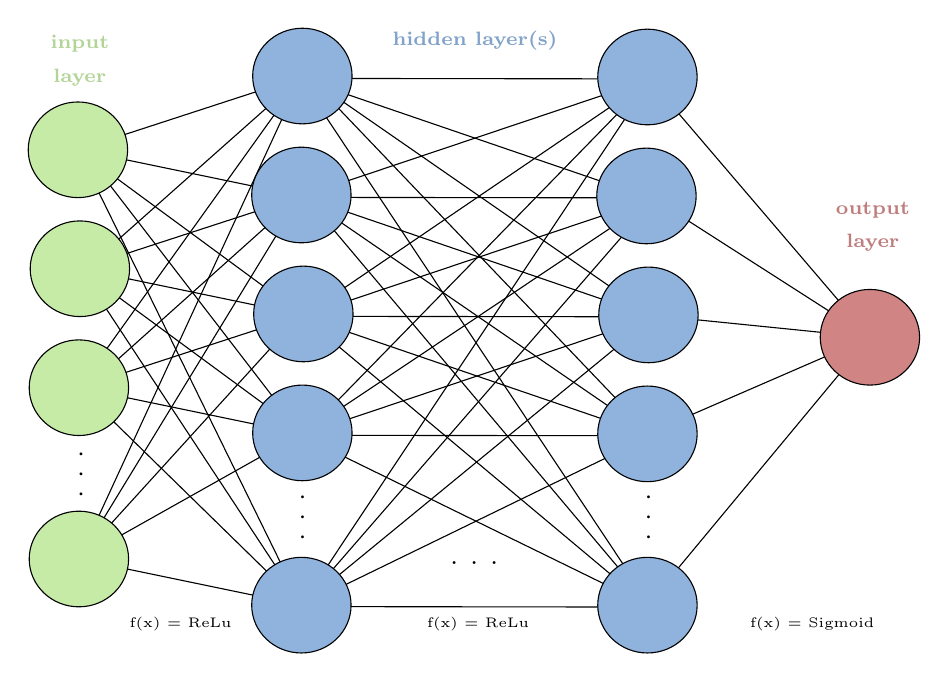
\begin{tikzpicture}[x=0.5pt,y=0.5pt,yscale=-1,xscale=1]
      %uncomment if require: \path (0,496); %set diagram left start at 0, and has height of 496

      %Straight Lines [id:da3125603624631026] 
      \draw    (205.85,243.68) -- (456.31,453.44) ;
      %Straight Lines [id:da4017136284587772] 
      \draw    (44.71,124.36) -- (206.2,71.74) ;
      %Straight Lines [id:da2227878135161746] 
      \draw    (46.14,210.32) -- (207.63,157.71) ;
      %Straight Lines [id:da35416891916640736] 
      \draw    (45.42,296.29) -- (206.92,243.68) ;
      %Straight Lines [id:da16193112504220186] 
      \draw    (45.42,420.09) -- (206.2,329.65) ;
      %Straight Lines [id:da3497039034753928] 
      \draw    (44.71,124.36) -- (205.49,157.71) ;
      %Straight Lines [id:da24573604202629373] 
      \draw    (46.14,210.32) -- (206.92,243.68) ;
      %Straight Lines [id:da01718938654762414] 
      \draw    (45.42,296.29) -- (206.2,329.65) ;
      %Straight Lines [id:da4694218304226967] 
      \draw    (45.42,420.09) -- (206.2,453.44) ;
      %Straight Lines [id:da6780505366621903] 
      \draw    (44.71,124.36) -- (206.92,243.68) ;
      %Straight Lines [id:da3700806633588325] 
      \draw    (46.14,210.32) -- (208.35,329.65) ;
      %Straight Lines [id:da7204661169538961] 
      \draw    (45.42,296.29) -- (206.2,453.44) ;
      %Straight Lines [id:da03352111792760715] 
      \draw    (49.89,126.59) -- (206.2,329.65) ;
      %Straight Lines [id:da7880697711535636] 
      \draw    (44.71,124.36) -- (206.2,453.44) ;
      %Straight Lines [id:da8177807044758987] 
      \draw    (46.14,210.32) -- (206.2,453.44) ;
      %Straight Lines [id:da5902292990985858] 
      \draw    (49.89,210.5) -- (206.2,71.74) ;
      %Straight Lines [id:da7293359024356544] 
      \draw    (45.42,296.29) -- (206.2,71.74) ;
      %Straight Lines [id:da8672682409124693] 
      \draw    (45.42,420.09) -- (206.2,71.74) ;
      %Straight Lines [id:da14015258542164877] 
      \draw    (52.03,295.09) -- (205.49,157.71) ;
      %Straight Lines [id:da6510778766409582] 
      \draw    (45.42,420.09) -- (205.49,157.71) ;
      %Straight Lines [id:da19048953930291812] 
      \draw    (45.42,420.09) -- (205.85,243.68) ;
      %Straight Lines [id:da5900414918521127] 
      \draw    (205.52,72.77) -- (459.29,73.12) ;
      %Straight Lines [id:da9923475282888197] 
      \draw    (204.06,158.74) -- (459.29,73.12) ;
      %Straight Lines [id:da6224502087859033] 
      \draw    (206.98,244.71) -- (462.21,159.09) ;
      %Straight Lines [id:da21387151774072322] 
      \draw    (205.52,330.68) -- (460.75,245.05) ;
      %Straight Lines [id:da40912543404428503] 
      \draw    (205.52,454.47) -- (459.29,331.02) ;
      %Straight Lines [id:da6756606943081097] 
      \draw    (208.44,158.74) -- (462.21,159.09) ;
      %Straight Lines [id:da16137493446626694] 
      \draw    (206.98,244.71) -- (460.75,245.05) ;
      %Straight Lines [id:da10150687813127202] 
      \draw    (205.52,330.68) -- (459.29,331.02) ;
      %Straight Lines [id:da0030866090013578207] 
      \draw    (205.52,454.47) -- (459.29,454.82) ;
      %Straight Lines [id:da5047969586038915] 
      \draw    (206.98,244.71) -- (459.29,73.12) ;
      %Straight Lines [id:da16781805884673007] 
      \draw    (204.43,334.29) -- (459.29,73.12) ;
      %Straight Lines [id:da5565130910620758] 
      \draw    (205.52,454.47) -- (459.29,73.12) ;
      %Straight Lines [id:da36371826499194726] 
      \draw    (205.52,454.47) -- (462.21,159.09) ;
      %Straight Lines [id:da11821496918512042] 
      \draw    (205.52,330.68) -- (462.21,159.09) ;
      %Straight Lines [id:da7692636391915034] 
      \draw    (205.52,72.77) -- (457.83,159.09) ;
      %Straight Lines [id:da6770318174394677] 
      \draw    (208.44,158.74) -- (460.75,245.05) ;
      %Straight Lines [id:da9309923147992141] 
      \draw    (206.98,244.71) -- (459.29,331.02) ;
      %Straight Lines [id:da7413198534186101] 
      \draw    (213.18,73.63) -- (460.75,245.05) ;
      %Straight Lines [id:da26068921273410117] 
      \draw    (213.18,73.63) -- (459.29,331.02) ;
      %Straight Lines [id:da8585525579192329] 
      \draw    (205.52,72.77) -- (459.29,454.82) ;
      %Straight Lines [id:da2270863173532055] 
      \draw    (213.18,162.87) -- (459.29,454.82) ;
      %Straight Lines [id:da5864780819119888] 
      \draw    (205.52,330.68) -- (459.29,454.82) ;
      %Straight Lines [id:da16348930210331503] 
      \draw    (205.52,454.47) -- (460.75,245.05) ;
      %Straight Lines [id:da2425074417898001] 
      \draw    (208.44,158.74) -- (459.29,331.02) ;
      %Straight Lines [id:da13422732156968453] 
      \draw    (456.31,71.74) -- (617.09,259.84) ;
      %Straight Lines [id:da7308781194762678] 
      \draw    (457.74,157.71) -- (617.09,259.84) ;
      %Straight Lines [id:da5359704776892366] 
      \draw    (457.02,243.68) -- (617.09,259.84) ;
      %Straight Lines [id:da3406152128273612] 
      \draw    (456.31,329.65) -- (617.09,259.84) ;
      %Straight Lines [id:da14904168253418448] 
      \draw    (456.31,453.44) -- (617.09,259.84) ;
      %Shape: Ellipse [id:dp8560274429988182] 
      \draw  [fill={rgb, 255:red, 198; green, 235; blue, 167 }  ,fill opacity=1 ] (8.8,124.36) .. controls (8.8,105.27) and (24.88,89.8) .. (44.71,89.8) .. controls (64.54,89.8) and (80.62,105.27) .. (80.62,124.36) .. controls (80.62,143.44) and (64.54,158.91) .. (44.71,158.91) .. controls (24.88,158.91) and (8.8,143.44) .. (8.8,124.36) -- cycle ;
      %Shape: Ellipse [id:dp5971121909630736] 
      \draw  [fill={rgb, 255:red, 198; green, 235; blue, 167 }  ,fill opacity=1 ] (10.23,210.32) .. controls (10.23,191.24) and (26.31,175.76) .. (46.14,175.76) .. controls (65.97,175.76) and (82.05,191.24) .. (82.05,210.32) .. controls (82.05,229.41) and (65.97,244.88) .. (46.14,244.88) .. controls (26.31,244.88) and (10.23,229.41) .. (10.23,210.32) -- cycle ;
      %Shape: Ellipse [id:dp024903598729203225] 
      \draw  [fill={rgb, 255:red, 198; green, 235; blue, 167 }  ,fill opacity=1 ] (9.51,296.29) .. controls (9.51,277.21) and (25.59,261.73) .. (45.42,261.73) .. controls (65.25,261.73) and (81.33,277.21) .. (81.33,296.29) .. controls (81.33,315.38) and (65.25,330.85) .. (45.42,330.85) .. controls (25.59,330.85) and (9.51,315.38) .. (9.51,296.29) -- cycle ;
      %Shape: Ellipse [id:dp2752980849146809] 
      \draw  [fill={rgb, 255:red, 198; green, 235; blue, 167 }  ,fill opacity=1 ] (9.51,420.09) .. controls (9.51,401) and (25.59,385.53) .. (45.42,385.53) .. controls (65.25,385.53) and (81.33,401) .. (81.33,420.09) .. controls (81.33,439.17) and (65.25,454.64) .. (45.42,454.64) .. controls (25.59,454.64) and (9.51,439.17) .. (9.51,420.09) -- cycle ;

      %Shape: Ellipse [id:dp22212680764969794] 
      \draw  [fill={rgb, 255:red, 143; green, 179; blue, 221 }  ,fill opacity=1 ] (171.01,71.06) .. controls (171.01,51.97) and (187.09,36.5) .. (206.92,36.5) .. controls (226.75,36.5) and (242.83,51.97) .. (242.83,71.06) .. controls (242.83,90.14) and (226.75,105.61) .. (206.92,105.61) .. controls (187.09,105.61) and (171.01,90.14) .. (171.01,71.06) -- cycle ;
      %Shape: Ellipse [id:dp31615925311964466] 
      \draw  [fill={rgb, 255:red, 143; green, 179; blue, 221 }  ,fill opacity=1 ] (170.3,157.02) .. controls (170.3,137.94) and (186.37,122.46) .. (206.2,122.46) .. controls (226.04,122.46) and (242.11,137.94) .. (242.11,157.02) .. controls (242.11,176.11) and (226.04,191.58) .. (206.2,191.58) .. controls (186.37,191.58) and (170.3,176.11) .. (170.3,157.02) -- cycle ;
      %Shape: Ellipse [id:dp763257580789] 
      \draw  [fill={rgb, 255:red, 143; green, 179; blue, 221 }  ,fill opacity=1 ] (171.73,242.99) .. controls (171.73,223.9) and (187.8,208.43) .. (207.63,208.43) .. controls (227.47,208.43) and (243.54,223.9) .. (243.54,242.99) .. controls (243.54,262.08) and (227.47,277.55) .. (207.63,277.55) .. controls (187.8,277.55) and (171.73,262.08) .. (171.73,242.99) -- cycle ;
      %Shape: Ellipse [id:dp41332126656266754] 
      \draw  [fill={rgb, 255:red, 143; green, 179; blue, 221 }  ,fill opacity=1 ] (171.01,328.96) .. controls (171.01,309.87) and (187.09,294.4) .. (206.92,294.4) .. controls (226.75,294.4) and (242.83,309.87) .. (242.83,328.96) .. controls (242.83,348.05) and (226.75,363.52) .. (206.92,363.52) .. controls (187.09,363.52) and (171.01,348.05) .. (171.01,328.96) -- cycle ;
      %Shape: Ellipse [id:dp3269904901419234] 
      \draw  [fill={rgb, 255:red, 143; green, 179; blue, 221 }  ,fill opacity=1 ] (170.3,453.44) .. controls (170.3,434.35) and (186.37,418.88) .. (206.2,418.88) .. controls (226.04,418.88) and (242.11,434.35) .. (242.11,453.44) .. controls (242.11,472.53) and (226.04,488) .. (206.2,488) .. controls (186.37,488) and (170.3,472.53) .. (170.3,453.44) -- cycle ;
      %Shape: Ellipse [id:dp43598218516443177] 
      \draw  [fill={rgb, 255:red, 143; green, 179; blue, 221 }  ,fill opacity=1 ] (420.4,71.74) .. controls (420.4,52.66) and (436.48,37.18) .. (456.31,37.18) .. controls (476.14,37.18) and (492.22,52.66) .. (492.22,71.74) .. controls (492.22,90.83) and (476.14,106.3) .. (456.31,106.3) .. controls (436.48,106.3) and (420.4,90.83) .. (420.4,71.74) -- cycle ;
      %Shape: Ellipse [id:dp5839593265260355] 
      \draw  [fill={rgb, 255:red, 143; green, 179; blue, 221 }  ,fill opacity=1 ] (419.69,157.71) .. controls (419.69,138.62) and (435.76,123.15) .. (455.6,123.15) .. controls (475.43,123.15) and (491.5,138.62) .. (491.5,157.71) .. controls (491.5,176.8) and (475.43,192.27) .. (455.6,192.27) .. controls (435.76,192.27) and (419.69,176.8) .. (419.69,157.71) -- cycle ;
      %Shape: Ellipse [id:dp5046190422661424] 
      \draw  [fill={rgb, 255:red, 143; green, 179; blue, 221 }  ,fill opacity=1 ] (421.12,243.68) .. controls (421.12,224.59) and (437.19,209.12) .. (457.02,209.12) .. controls (476.86,209.12) and (492.93,224.59) .. (492.93,243.68) .. controls (492.93,262.77) and (476.86,278.24) .. (457.02,278.24) .. controls (437.19,278.24) and (421.12,262.77) .. (421.12,243.68) -- cycle ;
      %Shape: Ellipse [id:dp04717464708306185] 
      \draw  [fill={rgb, 255:red, 143; green, 179; blue, 221 }  ,fill opacity=1 ] (420.4,329.65) .. controls (420.4,310.56) and (436.48,295.09) .. (456.31,295.09) .. controls (476.14,295.09) and (492.22,310.56) .. (492.22,329.65) .. controls (492.22,348.73) and (476.14,364.21) .. (456.31,364.21) .. controls (436.48,364.21) and (420.4,348.73) .. (420.4,329.65) -- cycle ;
      %Shape: Ellipse [id:dp9408343992389916] 
      \draw  [fill={rgb, 255:red, 143; green, 179; blue, 221 }  ,fill opacity=1 ] (420.4,453.44) .. controls (420.4,434.35) and (436.48,418.88) .. (456.31,418.88) .. controls (476.14,418.88) and (492.22,434.35) .. (492.22,453.44) .. controls (492.22,472.53) and (476.14,488) .. (456.31,488) .. controls (436.48,488) and (420.4,472.53) .. (420.4,453.44) -- cycle ;
      %Shape: Ellipse [id:dp47294074537144504] 
      \draw  [fill={rgb, 255:red, 209; green, 132; blue, 132 }  ,fill opacity=1 ] (581.18,259.84) .. controls (581.18,240.75) and (597.26,225.28) .. (617.09,225.28) .. controls (636.92,225.28) and (653,240.75) .. (653,259.84) .. controls (653,278.93) and (636.92,294.4) .. (617.09,294.4) .. controls (597.26,294.4) and (581.18,278.93) .. (581.18,259.84) -- cycle ;
      % Text Node
      \draw (50,340) node [anchor=north west][inner sep=0.75pt]  [rotate=-90] [align=left] {. . .};
      % Text Node
      \draw (210,371) node [anchor=north west][inner sep=0.75pt]  [rotate=-90] [align=left] {. . .};
      % Text Node
      \draw (460,371) node [anchor=north west][inner sep=0.75pt]  [rotate=-90] [align=left] {. . .};
      % Text Node
      \draw (312,420) node [anchor=north west][inner sep=0.75pt]  [rotate=0] [align=left] {. . .};
      % Text Node
      \draw (22,39.75) node [anchor=north west][inner sep=0.75pt]  [color={rgb, 255:red, 198; green, 235; blue, 167 }  ,opacity=1 ] [align=left] {\begin{minipage}[lt]{22.16pt}\setlength\topsep{0pt}
      \begin{center}
      {\scriptsize \textcolor[rgb]{0.7,0.83,0.59}{\textbf{input\\layer}}}
      \end{center}

      \end{minipage}};
      % Text Node
      \draw (270.19,36.82) node [anchor=north west][inner sep=0.75pt]   [align=left] {{\scriptsize \textcolor[rgb]{0.51,0.64,0.79}{\textbf{hidden layer(s)}}}};
      % Text Node
      \draw (590.42,160.07) node [anchor=north west][inner sep=0.75pt]   [align=left] {\begin{minipage}[lt]{26.92pt}\setlength\topsep{0pt}
      \begin{center}
      {\scriptsize \textbf{\textcolor[rgb]{0.75,0.49,0.49}{output\\layer}}}
      \end{center}

      \end{minipage}};
      % Text Node
      \draw (80.17,460) node [anchor=north west][inner sep=0.75pt]   [align=left] {{\tiny f(x) = ReLu}};
      % Text Node
      \draw (295.11,460) node [anchor=north west][inner sep=0.75pt]   [align=left] {{\tiny f(x) = ReLu}};
      % Text Node
      \draw (528.6,460) node [anchor=north west][inner sep=0.75pt]   [align=left] {{\tiny f(x) = Sigmoid}};


   \end{tikzpicture}
   \caption[Neural Network Architecture]{Architecture of the NN used on this thesis. 
   The neurons on the hidden layer(s) is a hyperparameter, as well as the number of hidden layers. }\label{fig:NNArch}
\end{figure}
\\Making this type of NN using \verb|TensorFlow| is easy. An algorithm showing one of the possibilites can be seen in Algorithm \ref{alg:nn}.
\begin{lstlisting}[language=Python, caption={Neural network definition using TensorFlow}, label=alg:nn, captionpos=t]
   import tensorflow as tf
   from tensorflow.keras import layers
   
   def Neural_Network(inputsize, n_layers, n_neuron, eta, lamda):
       
       model=tf.keras.Sequential()      
       
       for i in range(n_layers):       
           if (i==0):                  
               model.add(layers.Dense(n_neuron, activation='relu', kernel_regularizer=
                tf.keras.regularizers.l2(lamda), input_dim=inputsize))
           else:                       
               model.add(layers.Dense(n_neuron, activation='relu', kernel_regularizer=
                       tf.keras.regularizers.l2(lamda)))
                       
       model.add(layers.Dense(1,activation='sigmoid')) 
       
       sgd=tf.optimizers.SGD(learning_rate=eta)
       
       model.compile(loss=tf.losses.BinaryCrossentropy(),
                   optimizer=sgd,
                   metrics = [tf.keras.metrics.BinaryAccuracy()])
       return model
   \end{lstlisting}
To get the best performance on our NN, we need to find which hyperparemters helps the network reach highest significance. To do this, we need to do a gridsearch. 
For our neural network we will mainly focus on four hyperparameters explained on section \ref{sec:theory_nn}:
\begin{itemize}
   \item The learning rate $\eta$
   \item The L2-regressor variable $\lambda$
   \item The number of neurons on each hidden layer \verb|n_neuron|
   \item Possibly the number of layers \verb|n_layers|, exluding the output. Meaning that \verb|n_layers| = 1 means no hidden layer
\end{itemize}
The metrics that will be used to estimate the best hyperparameters are \textbf{AUC}, \textbf{binary accuracy} and most importantly \textbf{expected significance}. 
The expected significance for this section has been calculated using the low statistics formula Eq. (\ref{eq:exp_sig}) without uncertainties. The expected significance will also be calculcated when making a cut on 0.85 on the network prediction score, as explained in Chapter \ref{sec:siggy}. 
Meaning we will only look at events which the network rates as signal with 85\% confidence and above. For some models where the expected events are too low (EFT models), meaning that the expected significance will be 0 or \verb|NaN|, if this happens we will use the hyperparemeters of the network 
which gives us the highest AUC on the testing set. This will precedure will be done for every single network we will explore.
\clearpage


\section{Boosted Desicion Tree Training}
When working with BDTs we do not run into as many problems as we do with NNs. For example the padding and normalization of data can be completely avoided, making the whole procedure a lot easier when one uses exotic data as we do in high energy particle physics.
The weights is still an obstacle that needs to be overcome when using BDTS. This will be discussed in the next section.\\
\\For this project we will as mentioned utilize the eXtreme Gradient Boosting, or \verb|XGBoost| for short, package \cite{XGBoost} made for the Higgs ML Challenge \cite{HiggsChallenge} whenever we mention BDTs.
This project utilized version \verb|1.5.0| without GPU adaptability. \verb|XGBoost| also helps to avoid padding as it is integrated with a \verb|missing_variable| variable where we can simply write the number of the variable that is missing.

\subsection{Sample weights}
For \verb|XGBoost| there is a different problem when it comes to weights. XGBoost has a variable called \verb|scale_pos_weight| where we can help the network deal with unbalanced data, such as the one we have. 
Meaning that the whole problem of combining the re-weighting weights with the balancing weights from Chapter \ref{sec:sample_wgts_NN} completely dissapears. Albeit there is a caveat, \verb|XGBoost| does not have to possibility to include negative weights, which this dataset has. The reason \verb|XGBoost| 
doesn't include weights is because when calculating the number of events in a leaf node, which is made by taking the sum of sample weights, we cannot have a negative value \cite{neg_wgt_xbg1, neg_wgt_xbg2}.
As for the MC generators, Sherpa \cite{Sherpa} takes into acount higher order diagrams and needs to add negative weights to "counter" the overcounting of diagrams \cite{Negative_Weights_article}, which are important to correctly scale the simulated events to real data.
In the future this might no longer be a problem as \todo{I have no other sources to this other than spoken words at conferenes...} future MC generators might only have positive weights.\\
\\A method to mitigate this problem is to use the absolute value of the weights when training. This is however not generally accepted as a solution, and some even say it should be avoided. There are other options however, one of these options is to not include events with negative weights on the training set. 
This is an okay thing to do, as we can imagine that if we were to only include events with positive weights on the training, it might be the same as putting the negative weights on the "testing dataset" (Chapter \ref{sec:train_test}). \\
\\Another one that has been used on a published ATLAS (internal) article (chapter 9.3) \cite{Abbott:2714377} is to normalize the weights when using the absolute value with respect to the sum of weights over the sum of absolute weights. The reason behind this is because the sum of weights is obviously not the same when we take the absolute value. 
Mathemathically speaking, if we have an array of weights $W$, we can update this like
\begin{equation}\label{eq:ATLAS_wgt}
   W \rightarrow \abs{W}\frac{\sum_i W_i}{\sum_i\abs{W_i}}
\end{equation}
such that the weights are at least in the same scale. 

\subsection{Architecture and hyperparameter tuning}\label{sec:BDTGriddy}
Making a BDT for our purposes is fairly easy as well using XGBoost. One way to do it is using the code below in Algorithm \ref{alg:xgb}
\begin{lstlisting}[language=Python, caption={Boosted Decision Tree definition using XGBoost}, label=alg:xgb, captionpos=t]
   import xgboost as xgb
   
   Boosted_Decision_Tree = xgb.XGBClassifier(
                max_depth, 
                use_label_encoder=False,
                n_estimators,
                learning_rate,
                reg_lambda,
                predictor = 'cpu_predictor',
                tree_method = 'hist',
                scale_pos_weight = sow_bkg/sow_sig,
                objective = 'binary:logistic',
                eval_metric = 'auc',
                min_child_weight = 1,
                missing = -999,
                random_state = 42,
                verbosity = 1) 
\end{lstlisting}
To get the best performance on our BDT we have to do a grid search here as well. The trainable hyperparameters here are different than for NNs though. With XGBoost we have the following hyperparameters
\begin{itemize}
   \item Tree depth: how many times we split the data
   \item Number of estimators: how many trees we use to do the gradient boosting
   \item The learning rate $\eta$
   \item L2-regressor $\lambda$, to stop overtraning
\end{itemize}
The metrics that will be used to estimate the best hyperparameters are \textbf{AUC}, \textbf{binary accuracy} and most importantly \textbf{expected significance}. 
The expected significance for this section has been calculated using the low statistics formula Eq. (\ref{eq:exp_sig}) without uncertainties. The expected significance will also be calculcated when making a cut on 0.85 on the network prediction score, as explained in Chapter \ref{sec:siggy}. 
Meaning we will only look at events which the network rates as signal with 85\% confidence and above. For some models where the expected events are too low (EFT models), meaning that the expected significance will be 0 or \verb|NaN|, if this happens we will use the hyperparemeters of the network 
which gives us the highest AUC on the testing set. This will precedure will be done for every single network we will explore.

\end{document}